\section{\LaTeX}

{\setbeamertemplate{background canvas}{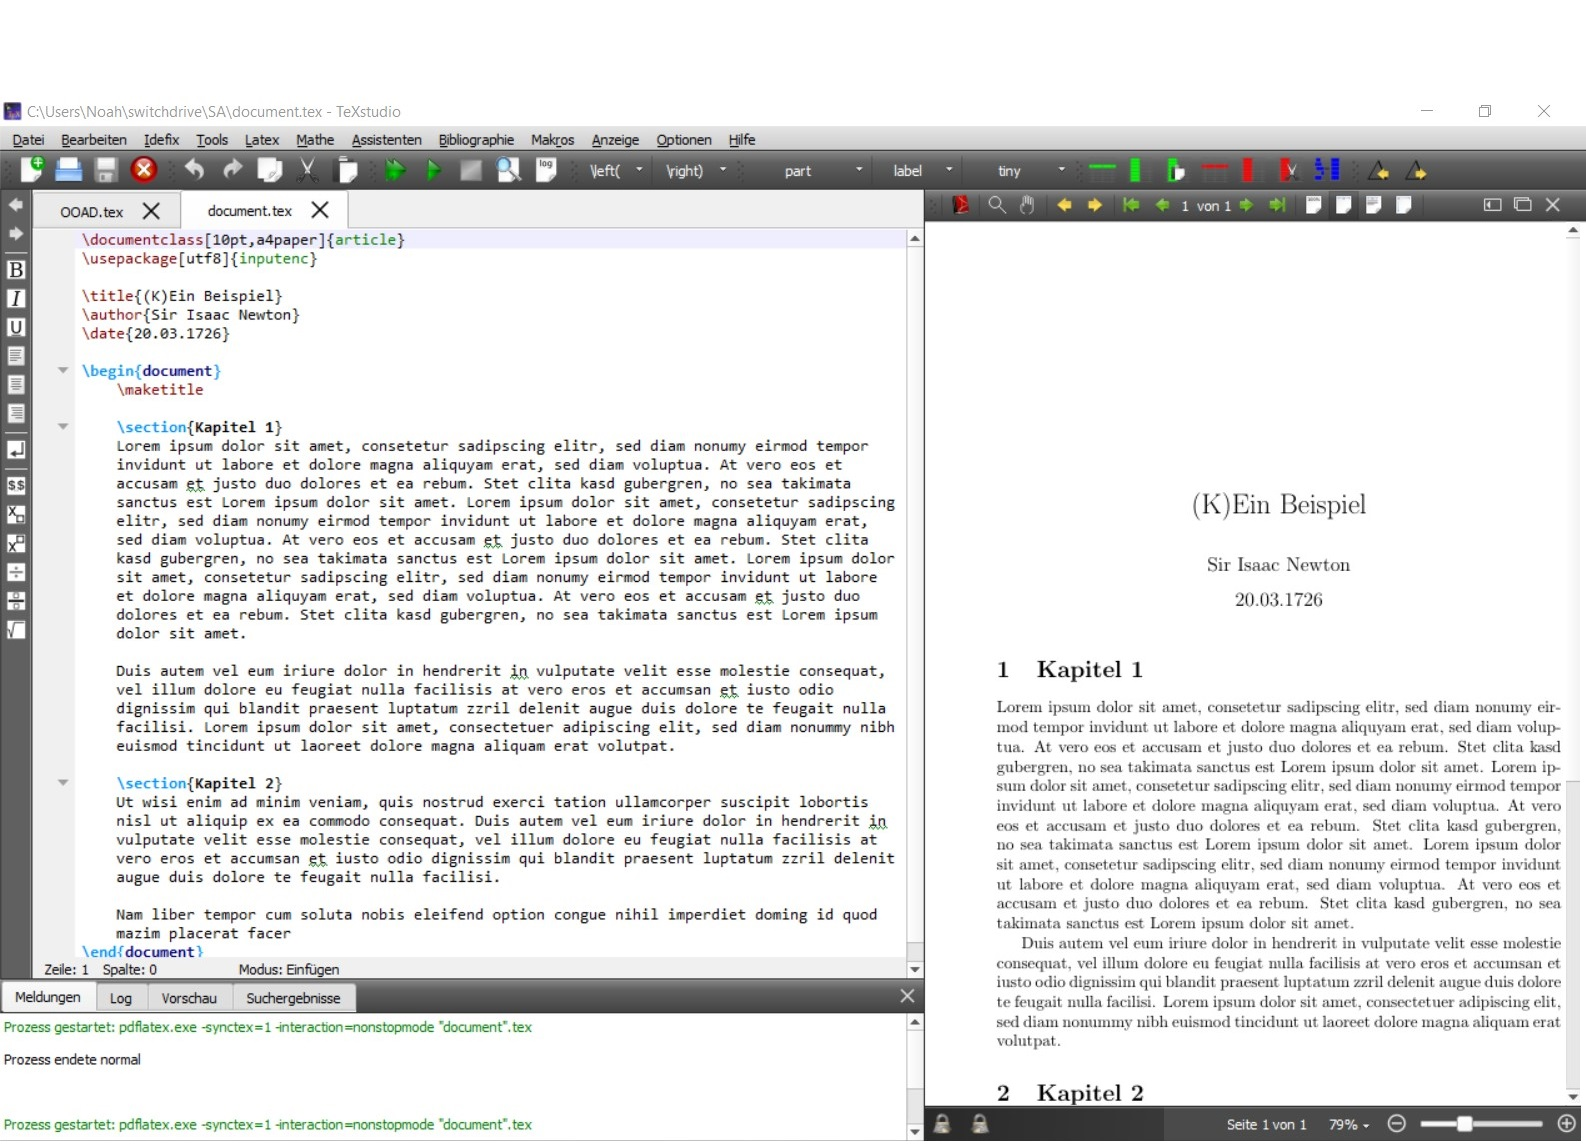
\includegraphics[width=\paperwidth]{pic/bild}}
\begin{frame}

\end{frame}
}

\begin{frame}{Was ist \LaTeX}
	\begin{itemize}
		\item \LaTeX: \textbf{La}mport \textbf{TeX} \pause
		\item TeX: Textsatzsystem  \pause
		\item Kein WYSIWYG sondern WYSIWYAF
	\end{itemize}
\end{frame}

\begin{frame}{Warum \LaTeX?}
\begin{itemize}
	\item Open-Source  \pause
	\item Grosse Community  \pause
	\item Performance  \pause
	\item Kein WYSIWYG  \pause
	\item Professionell  \pause
	\item Wissenschaftliche Formeln  \pause
	\item Cross-Platform
\end{itemize}
\end{frame}
